This chapter presents the results of the experiment and associated data collection
methods mentioned in~\ref{chap:method}.

\subsection{Survey}

\subsubsection{Pre-Survey}
The pre-survey focused on two aspects: it should capture the students' previous
programming experience, and it should gauge their confidence in explaining four
selected software design concepts.

All students reported previous programming experience. Condidence in being able to
solve complex programming tasks was low. However, all students indicated that they
had some experience in using a visual programming language (Scratch). Further, both
the Scratch student and one of the Godot Orchestrator students said that they had
programmed in a textual programming language before too. Regarding the to-be-analyzed
programming concepts (modularity, instantiation, state management, event handling),
confidence in explaining any of them was rather low, with the exception of instantiation.

The Scratch student indicated both the most experience with programming and the
highest confidence in explaining the different programming concepts: instantiation
and event handling were rated higher than modularity and state management, however
the student was still confident in explaining the latter concepts too.

The two Godot Orchestrator students varied in their experience. One student reported
some programming experience, mostly visual-based programming. The other student seemed
to have considerable programming experience, even with creating games. The latter
had used more textual programming languages than visual programming languages in the
past. Overall, both Godot Orchestrator students indicated low confidence in explaining
any of the four programming principles.

\subsubsection{Post-Survey}
The post-survey focused on two aspects: it should capture the students' experience
with their respective visual programming language during the workshop, and it should
again gauge their confidence in explaining the same four selected software design
concepts as in the pre-survey.

Independently of which VPL they used, students reported high confidence in building
large programs with their respective VPL. Confidence in solving complex problems
with VPLs was reported low similar to the pre-survey results. Taken together, students
using either of the two languages reported that their language might help with
addressing modularity in their code, however they saw problems for state management.
Results for event handling and instantiation were mixed. Contrary, confidence in
explaining was highest in event handling and state management, with mixed results for
modularity and instantiation.

The Scratch student evaluated Scratch's ability to achieve modularity, instantiation
and event handling as high, whereas state management seemed harder in Scratch. In
addition, the Scratch student indicated increased confidence in explaining any of
the four concepts, compared to the results of the pre-survey. The other students saw
Godot Orchestrator's ability to implement the different concepts more critical. One
student did not find the language useful for implementing any of the four concepts.
The other student found it at least useful for modularity and instantiation.

Regarding their confidence in explaining the four concepts it was lower than what
the Scratch user reported. One Godot Orchestrator reported low confidence in explaining
any of the concepts. The other student answers with high confidence in explaining event
handling. State management was rated neutral from both Godot Orchestrator students. In
sum, the questions regarding whether the respective language helps implementing
programming concepts yield contrary results to the questions about student confidence
in explaining the same concepts.

Fig. \ref{fig:pre-post-survey} shows pre-survey answers mapped to their post-survey
equivalents. It shows how confident students were explaining in each of the four
concepts. All data points left of the diagonal line show an improvement, whereas all
data points on the right indicate that confidence went down. Of the four concepts only
instantiation stagnated or even decreased, whereas the others mostly improved for both
Scratch and Godot users. Overall, the understanding of state management and event
handling seem to have improved most, according to the surveys.

\begin{figure}[htbp]
    \centering
    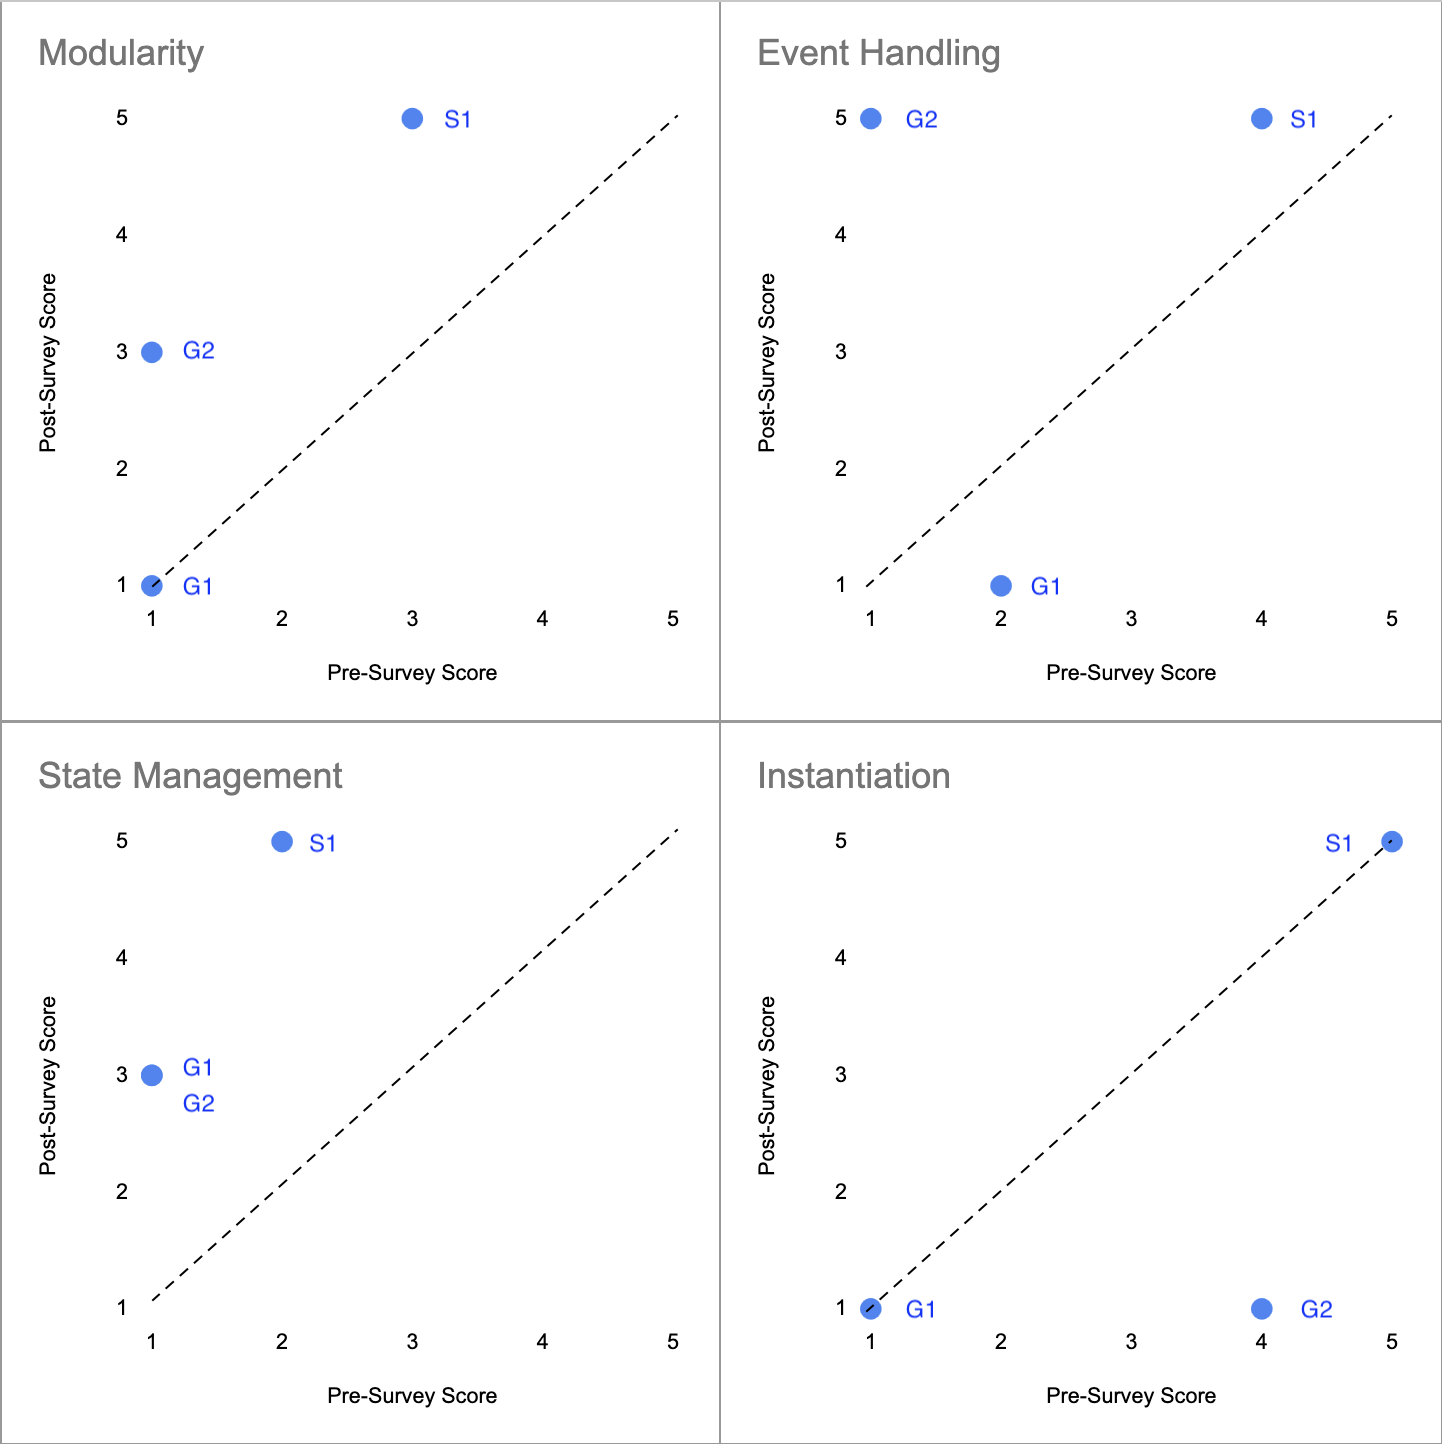
\includegraphics[width=\linewidth]{images/pre-post-survey}
    \caption{Pre- and post-survey answers for each participant (S1: Scratch, G1+G2: Godot)}
    \label{fig:pre-post-survey}
\end{figure}

As Fig. \ref{fig:confidence-change} suggests, both visual programming languages
performed differently in conveying the four concepts. Based on the collected survey
answers, Scratch seems to have better explained state management, whereas Godot
Orchestrator positively influenced the students' confidence in explaining event
handling. Modularity worked well in both languages, and instantiation appears hard to
grasp in Godot Orchestrator. Scratch on the other hand seemed to have no effect
on the students' confidence in explaining instantiation, which was already high in
the pre-survey. Overall, both languages seem to have improved the students' confidence
in explaining the software design concepts.

\begin{figure}[htbp]
    \centering
    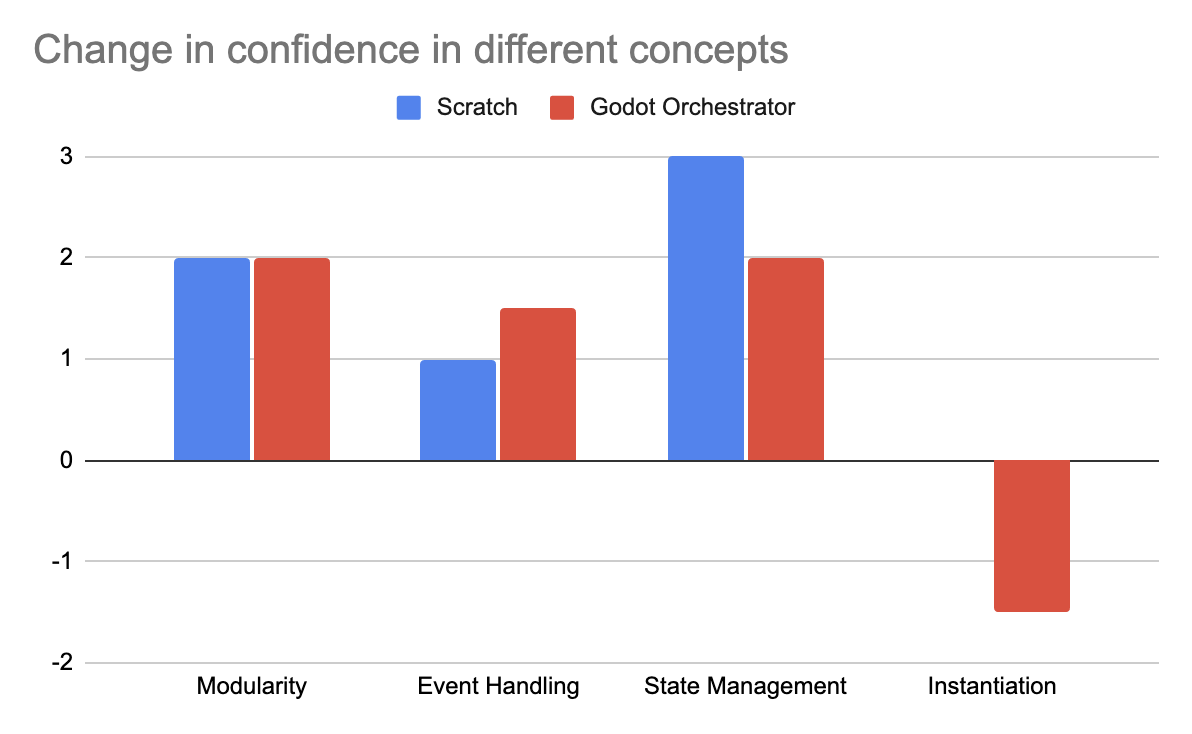
\includegraphics[width=\linewidth]{images/confidence-change}
    \caption{Change in confidence in different concepts}
    \label{fig:confidence-change}
\end{figure}

\subsection{Multiple Choice Test}
Due to an organizational mistake, we only conducted the multiple choice test after
the workshop, instead of both before and after. The actual idea was to run the same
test two times to achieve comparability. This is described in more detail in
\ref{chap:method}. Acknowledging our mistake, we still want to present the results of
the post test.

Overall, the Scratch student scored considerably higher than both Godot Orchestrator
students. While the Scratch student answered 50\% of the questions correctly, the
Godot Orchestrator students scored 20\% and 0\% respectively. The latter succeeded
only with state management-related questions, whereas the former had correct answers
related to modularity, event handling and state management. None of the students
answered any question concerning instantiation correctly. Across all students
modularity and state management were more successful than instantiation and event
handling.

As we did not conduct the pre multiple choice test there is no direct comparison
possible. However, we can relate the test results to the survey results mentioned
before. Instantiation was reported to be the most difficult concept during pre-
survey, which aligns with the low test results. The Scratch student reported high
confidence in explaining instantiation, however they still scored 0 points with
instantiation-related questions.

Modularity and state management were initially rated difficult too, however the post
survey showed an increase in confidence. The Scratch student indicated a better
understanding of those two concepts, and scored on related questions. One of the
Godot Orchestrator students did not feel improvement, which was accordingly reflected
in their test results (i.e., they scored 0\%). The other student reported a smaller
improvement than the Scratch student, however they only answered state management-
related questions correctly. While this aligns with the survey results regarding their
confidence in explaining state management, it does not reflect their confidence
increase regarding modularity.

Event handling seems overall to have been a hard to grasp concept in our workshop.
The Scratch student answered answered one of the two related questions correctly,
whereas both Godot Orchestrator students struggled with both questions. Those results
are contrary to the post survey results saying that two of the students had high
confidence in understanding the concept. It also somewhat contradicts the finding that
the confidence in explaining event handling increased the second most from pre- to
post-survey. It however aligns mostly with the pre-survey evaluation of event
handling, which described it as a difficult topic.

\subsection{Workshop Observation}
While conducting the programming workshop, including lecture and project work, we
took notes of the students' interaction with their respective visual programming
language. Again, we split our observations and map them to the four teaching concepts.
Further, we noted down observations regarding general usability issues. Overall,
only observations regarding modularity and instantiation could be made for the
Godot Orchestrator students, as they progressed slower in their projects than the
Scratch student.

Throughout the workshop the Scratch student showed a solid understanding of both
event handling and modularity. Without any further instruction, the student used
custom blocks to organize their codebase into smaller parts. Event handling was
intuitively used to capture user input. On the other hand, state management seemed
not well understood, even after multiple explanation attempts by the teacher.
Instantion was eventually used on the teacher's proposal. These observations somewhat
conform with the previous surveys and multiple choice test, as the Scratch student
indicated high confidence in explaining the concepts of modularity and event handling.
However, he also rated his understanding of the other concepts high (state management,
instantiation), which he seemed to struggle with within the project phase of the workshop.

The Godot students, despite only implementing two out of four design concepts, carefully
considered modularity and instantiation in their games. They appeared more disciplined
in using variables instead of hard-coded values, and they could both explain
verbally what instantiation would be used for in their projects. State management
and event handling were not tackled. Going from pre- to post-survey, there was in increase
in confidence in grasping modularity, which aligns with our observations. Understanding
of instantiation actually dropped from pre- to post-survey and was also never answered
correctly in the multiple choice test by any Godot Orchestrator student, which is an
interesting contrast compared to our observations, where they used instantiation
appropiatly.

\subsubsection{Modularity}
The concept of modularity was used to different degrees, if comparing Scratch and
Godot Orchestrator students. In general, the students using Godot Orchestrator seemed
to consider reuse of code more than the student using Scratch. Both Godot Orchestrator
showed a basic understanding of variables and functions, and considered them while
working on their projects. It also seemed like that they at least partly understood why
using variables instead of hard-coded values can be desirable. Similarly, the Scratch
student was aware of what variables and functions are and how they could be used in theory.
The student used functions (custom blocks) early in the project to organize their code.
However, it seemed like the student did not consider using variables and functions to
reuse code throughout their code base at this point. A teacher intervention, explaining
the benefits of reusing code, nudged the student into the desired direction.

\subsubsection{Instantiation}
Instantiation seemed to be well-understood in theory, i.e. when lecturing the students
and asking them related questions, but it was a challenging concept to grasp when working
with Scratch and Godot Orchestrator. The Scratch student initially implemented gun shooting
without using instantiation, but instead reused the same bullet object over and over
by temporarily hiding it and bringing it back to the gun. This worked because of the
cooldown time between each shot. Asking the student about how to enable rapid shooting
nudged them into switching over to a instantiation-based solution. One of the two Godot
Orchestrator students managed to implement instantiation for gun shooting following the
provided instructions. The other student did not get to implement the shooting mechanism,
and also did not use instantiation for any other feature. However, both could give an
explanation the concept when being asked about it.

\subsection{Event Handling}
Event Handling was explained during the short lecture as all other concepts, but only
the Scratch student progressed far enough to implement an event handling-related feature.
The Godot Orchestrator did not attempt building such feature due to time constraints.
The Scratch student intuitively used event handling when listening for keyboard input,
e.g., when checking press of arrow keys for player movement. An interesting observation
was that the student did not use Scratch's way of registering key press events, but
instead opted for a solution using a for loop that constantly checked for the player
input using a nested if statement. While leading to the same result, this deviated from
Scratch's standard way of registering key events. The same “long-polling” approach was
used when implementing collision detection. Lastly, the student used event handling when
implementing a level system, that would spawn multiple waves of enemies - this required
a more extensive teacher intervention though.

\subsubsection{State Management}
Similar to Event Handling, State Management was part of the lecture, where the concept
was explained to the students and the students asked questions. During the project phase,
where students worked on their projects, again only the Scratch student managed to attempt
implementing state management. This concept was seen as the most challenging to grasp,
and thus was explained multiple times to the student. Per project curriculum, it was
planned to use state management to map the different states of the weapon as a state
machine. Despite multiple teacher interventions the student did not succeed with
implementing a finite state machine.

\subsection{Usability}
The students expressed both wins and challenges when using Scratch or Godot Orchestrator.
While students were content with using functions in Godot Orchestrator, custom blocks in
Scratch were not intuitively desirable. The Godot Orchestrator students seemed to be happy
with refactoring their code into multiple functions. The Scratch student used custom blocks
to structure the code too, but did not show any positive reaction towards reuse of code.
The Godot Orchestrator students struggled more with using their code editor than the Scratch
student. Whereas the former especially struggled with finding the correct nodes to write their
scripts, the latter navigated the Scratch editor fluently and found blocks fast based on their
block category. The Godot Orchestrator students reported that it was hard to find nodes because
of high amount of nodes in Godot and because they did not know the name of most nodes.
Further, these students showed challenges with understanding nodes, that were related to
mathematical concepts like vectors. Further, there was confusion in Godot Orchestrator
regarding defining and setting variables in different places throughout the code base.